%%
%%
%%   LaTeX Beamer for ESS Presentation template
%%
%%   Jeong Han Lee, han.lee@esss.se
%%
%%   v0.1 created Monday, Monday, November 23 09:07:19 CET 2015, jhlee
%%
%%

\documentclass[
  9pt
  , table
  , ignorenonframetext
]{beamer}


\usepackage{esspre} 

\meetingname{PDR Target Imaging}
\meetingcity{Lund}
\meetingcountry{Sweden}
\totalpagenumber{\inserttotalframenumber}
%\totalpagenumber{13+}



\title{ICS HW Platform; focus on Imaging}
\author{Jeong \textbf{Han} Lee on behalf of ICS}%\inst{1}}
\institute{
  Integrated Control System Division\\
  \textbf{ESS}, Sweden
}
\date{Sep 21, 2016}


\begin{document}
 
\begin{frame}[plain]
  \titlepage
\end{frame}


\begin{frame}{The Integrated Control System (ICS)}
  \begin{block}{ICS Scope}
    \begin{itemize}
    \item Conventional facilities control integration : power distribution, cooling water, etc
    \item The Accelerator control system
    \item The Neutron target control system
    \item EPICS layer for the neutron instruments (in cooperation with the colleagues from science directorate)
    \item Global systems : control network and servers, timing and event systems, and protection \& safety systems
    \end{itemize}
  \end{block}
  \begin{exampleblock}{Combination of}
    \begin{itemize}
    \item On-site developments 
    \item In-kind contributions (up to 50\% of total value)
    \end{itemize}
  \end{exampleblock}
\end{frame}



\begin{frame}{EPICS Environment}
  There is no generic EPICS environment, and each lab has its own environment historically. Historically, many labs use more than one EPICS release and drivers should be built for all EPICS releases in parallel
  \begin{block}{Loadable Driver Module (LDM) at PSI}
    \begin{itemize}
    \item Build drivers for multiple releases of EPICS, and load drivers dynamically from startup script.
    \item is used to run PSI machine since 2005, which is the first presentation in the community.
    \end{itemize}
  \end{block}

  \begin{exampleblock}{ESS EPICS Environment}
    \begin{itemize}
    \item has been evolved from LDM in cooperation with Dirk Zimoch at PSI.
    \item provides a collection of scripts to develop, build, and deploy an EPICS IOC.
    \item provides customized solutions to run different configurations at the same time and in the same machine, to test next releases of IOCs independently, and to switch the old and new versions of an IOC easily and quickly.
    \end{itemize}
  \end{exampleblock}
\end{frame}

\begin{frame}{HW \& IO Strategy}
  \begin{block}{Generic}
    \begin{itemize}
    \item{MTCA :} High-speed front-end processing \& Digital front-end platform 
    \item{EtherCAT :} Mid-range, beam synchronized I/O \& Distributed I/O \& Cross-system integration
    \item{PLC :} Siemens S7-1500 : Industrial, process I/O \& Safety systems, high reliability
    \end{itemize}
  \end{block}
 \begin{exampleblock}{Specific}
    \begin{itemize}
    \item Timing / Event System : Micro-Research Finland EVM (EVG, Dist) \& EVR
    \item Motion Control : Beckhoff TwinCAT for coordinated motion \& Open source master for single-axis, simple motion
    \item Serial \& Network-based devices : almost de-facto Standard MOXA 
    \item Cameras : GigE, 10GB, CameraLink 
    \end{itemize}
  \end{exampleblock}
  
\end{frame}


\begin{frame}{High-speed Digital Controller Board}
  \begin{itemize}
  \item MTCA.4 AMC, Xilinx FPGA (Kintex Ultrascale), CPU (Freescale QorIQ T2081), and modular (FMC/RTM) interfaces
  \item In-kind contribution from Switzerland (PSI) with an industry partner (IOxOS SA)
  \item Embedded Linux (ELDK) OS \& EPICS software
  \item FPGA source code available to all ESS partners and licensees (very liberal but not fully open source)
  \end{itemize}
  \begin{exampleblock}{Supported and Planned Modular Interfaces}
    \begin{itemize}
    \item{IOxOS SA :} ADC 3110/3111 (8CH, 16bit, 250MSPS)
    \item{IOxOS SA :} ADC 3112 (4CH, 12bit, 900MSPS / 2CH, 12bit, 1800MSPS)
    \item{IOxOS SA :} ADC 3117 (In : 20CH, 16bit, 5MSPS \& Out : 2CH, 16bit, 0$\sim\pm$10V)
    \item{d-tAcq Solutions : } ACQ420 FMC (4CH, 16$\sim$20bit, 1MSPS)
    \item{Faster Technology : } FM-S14 (whereby support is limited due to application-dependent)
    \item{In-kind project of Estonia : } EtherCAT slave FMC
    \end{itemize}
  \end{exampleblock}
\end{frame}

\begin{frame}{Middle-range I/O}
\begin{itemize}
\item High-end platform is expensive and centralized; Use only where needed
\item Some applications still need time synchronization; Especially in a pulsed machine! PLCs are not ideal (asynchronous cycle times)
\item EtherCAT is a good solution for this range
\end{itemize}

\begin{block}{EtherCAT, We}
\begin{itemize}
\item can use a typical Ethernet cable and Ethernet switch
\item can run its master on a PC or MTCA IOC 
\item can achieve several kHz loop times 
\item can reduce cabling (distributed I/O)
\item have many different types of I/O modules
\end{itemize}
\end{block}

\end{frame}



\begin{frame}{Selected SW Platform}
  \begin{itemize}
  \item CentOS 7 (currently 7.1 1503)
  \item Development Machine (EEE, OpenXAL, IPhyton, CSS)
  \item ESS EPICS Environment (Linux Kernel module, EPICS Device support, EPICS IOC)
  \item Archiver Appliance for signal archiving 
  \item Control System Studio (mostly User Interface, but more than)
  \item Scripting Environment (Jupyter - planned, IPhyton - current)
  \end{itemize}

\end{frame}


\begin{frame}{Questions?}

   Computers are useless. They can only give you answers.
   \begin{flushright}
     Pablo Picasso 
   \end{flushright}
   
   It is not enough for me to ask the question; I want to know how to answer the one question that seems to encompass everything I face: What am I here for?
   \begin{flushright}
    Abraham Joshua-Heschel
   \end{flushright}

   
\end{frame}



%% \begin{frame}{ICS Control System Fact}
%%   \begin{exampleblock}{until 2016.06}
%%     \begin{itemize}
%%     \item 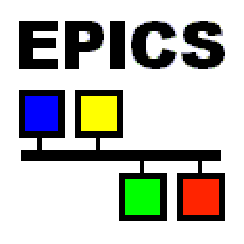
\includegraphics[width=0.06\textheight]{./pictures/epics_logo.eps}~ \textbf{EPICS}, and ESS EPICS Environment
%%     \item 
\includegraphics[width=0.05\textheight]{./pictures/centos-emboss.eps} ~ CentOS 64bit for OS (7.1  1503)
%%     \item 
\includegraphics[width=0.08\textheight]{./pictures/git_logo.eps}~ for sources version control 
%%     \item Event System : MRF EVG/EVR boards (cPCI, PCIe, VME, MTCA, etc)
%%     \item Siemens S7 PLC
%%     \item Control System Studio for OPI
%%     \end{itemize}
%%   \end{exampleblock}
%%   \end{frame}




%% \begin{frame}
%%   \frametitle{A Page for a picture}
%%   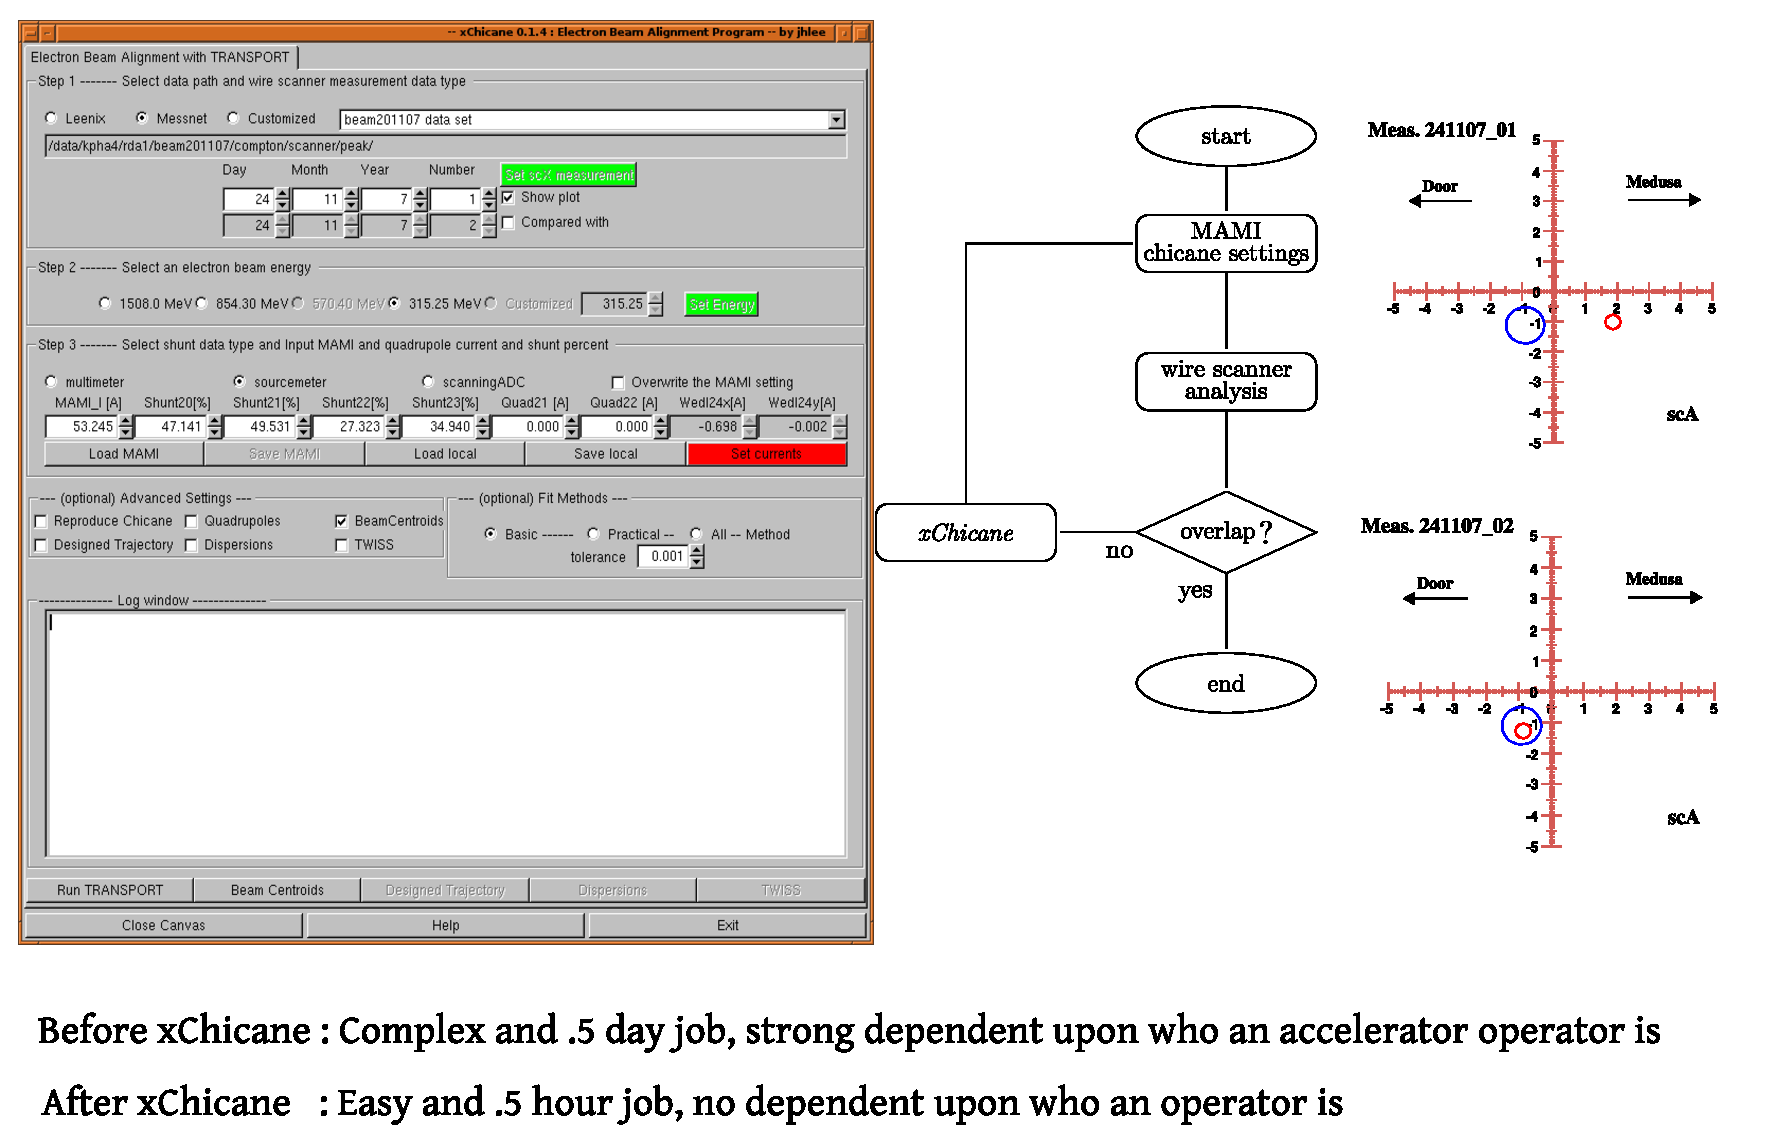
\includegraphics[width=\columnwidth]{./pictures/xchicane.eps}
%% \end{frame}


\begin{frame}[plain]
  \begin{center}
    {\LARGE Kiitos!}  \\\vspace{6mm}
    {\LARGE Tack!}  \\\vspace{6mm}
    {\LARGE Tak!}  \\\vspace{6mm}
    {\LARGE 감사합니다!}\\\vspace{6mm}
    {\LARGE Thank you!}  \\\vspace{6mm}
    {\LARGE Dankesch\"on!} \\\vspace{6mm}
%    {\LARGE ¡Gracias!}\\\vspace{6mm}
%    {\LARGE Grazie!}  \\\vspace{6mm}
%            {\LARGE Merci!}\\\vspace{6mm}
    {\LARGE \smiley } 
  \end{center}
  
\end{frame}



%% \begin{frame}{Motion Control - MPS integation}
%%   \begin{columns}
%%     \begin{column}{.6\textwidth}
%%       \begin{block}{MCU 1013 - Single Axis MPS version}
%%         \begin{itemize}
%%         \item CPU, couplier, linear stage, INC encoder, redundant switches
%%         \item Motion control with an Open Source EtherCAT master, which is being developed by ICS and the motion group at ESS
%%         \item Based on the open source EtherCAT technology
%%         \item The Open Source EtherCAT master (www.etherlab.org) can run on Linux
%%         \item  No software licences
%%           %%   \begin{itemize}
%%           %%   \item EtherCAT hardware have rather high performance
%%           %%   \item The Open Source EtherCAT master (www.etherlab.org) can run on Linux
%%           %%   \item No software licences
%%           %%   \item MCAG group also evaluates an industrial control system called TwinCAT (soft controller running under Windows operating system only) with EtherCAT hardware and the same hardware can be used with this open source approach
%%           %%   \item ICS is also using open source ethercat master (www.etherlab.org) for sampling analog and digital signals to EPICS. 
%%           %%   \end{itemize}
%%         \end{itemize}
%%       \end{block}
%%     \end{column}
%%     \begin{column}{.5\textwidth}
%%       \centering
%%       \includegraphics[width=1\textwidth]{./pictures/motion-ws-dual-axis.eps}
      
%%     \end{column}
%%     \end{columns}
%% \end{frame}

\end{document}
